\documentclass[a4paper]{article}
\usepackage[pdftex]{hyperref}
\usepackage[latin1]{inputenc}
\usepackage[english]{babel}
\usepackage{a4wide}
\usepackage{amsmath}
\usepackage{amssymb}
\usepackage{algorithmic}
\usepackage{algorithm}
\usepackage{ifthen}
\usepackage{listings}
\usepackage{xcolor}
% move the asterisk at the right position
\lstset{basicstyle=\ttfamily,tabsize=4,literate={*}{${}^*{}$}1}
%\lstset{language=C,basicstyle=\ttfamily}
\usepackage{moreverb}
\usepackage{palatino}
\usepackage{multicol}
\usepackage{tabularx}
\usepackage{comment}
\usepackage{verbatim}
\usepackage{color}
\usepackage{enumitem}
\usepackage{tikz}
\usetikzlibrary{arrows,shapes.gates.logic.US,shapes.gates.logic.IEC,calc}

\usepackage[left=3cm, right=3cm, top=4cm, bottom=4cm]{geometry}

\usepackage{graphicx}

%% pdflatex?
\newif\ifpdf
\ifx\pdfoutput\undefined
\pdffalse % we are not running PDFLaTeX
\else
\pdfoutput=1 % we are running PDFLaTeX
\pdftrue
\fi
\ifpdf
\ifpdf
\DeclareGraphicsExtensions{.pdf, .jpg}
\else
\DeclareGraphicsExtensions{.eps, .jpg}
\fi

\parindent=0cm
\parskip=0cm

\setlength{\columnseprule}{0.4pt}
\addtolength{\columnsep}{2pt}

\addtolength{\textheight}{5.5cm}
\addtolength{\topmargin}{-26mm}
\pagestyle{empty}

%%
%% Sheet setup
%% 
\newcommand{\coursename}{Computer Architecture and Programming Languages}
\newcommand{\courseno}{CO20-320241}
 
\newcommand{\sheettitle}{Homework}
\newcommand{\mytitle}{}
\newcommand{\mytoday}{November 25, 2019}

% Current Assignment number
\newcounter{assignmentno}
\setcounter{assignmentno}{10}

% Current Problem number, should always start at 1
\newcounter{problemno}
\setcounter{problemno}{1}

%%
%% problem and bonus environment
%%
\newcounter{probcalc}
\newcommand{\problem}[2]{
  \pagebreak[2]
  \setcounter{probcalc}{#2}
  ~\\
  {\large \textbf{Problem \arabic{assignmentno}.\arabic{problemno}} \hspace{0.2cm}\textit{#1}} \refstepcounter{problemno}\vspace{2pt}\\}

\newcommand{\bonus}[2]{
  \pagebreak[2]
  \setcounter{probcalc}{#2}
  ~\\
  {\large \textbf{Bonus Problem \arabic{assignmentno}.\arabic{problemno}} \hspace{0.2cm}\textit{#1}} \refstepcounter{problemno}\vspace{2pt}\\}

%% some counters  
\newcommand{\assignment}{\arabic{assignmentno}}

%% solution  
\newcommand{\solution}{\pagebreak[2]{\bf Solution:}\\}

%% Hyperref Setup
\hypersetup{pdftitle={Homework \assignment},
  pdfsubject={\coursename},
  pdfauthor={},
  pdfcreator={},
  pdfkeywords={Computer Architecture and Programming Languages},
  %  pdfpagemode={FullScreen},
  %colorlinks=true,
  %bookmarks=true,
  %hyperindex=true,
  bookmarksopen=false,
  bookmarksnumbered=true,
  breaklinks=true,
  %urlcolor=darkblue
  urlbordercolor={0 0 0.7}
}

\definecolor{mGreen}{rgb}{0,0.6,0}
\definecolor{mGray}{rgb}{0.5,0.5,0.5}
\definecolor{mPurple}{rgb}{0.58,0,0.82}
\definecolor{backgroundColour}{rgb}{0.95,0.95,0.92}

\lstdefinestyle{CStyle}{
    backgroundcolor=\color{backgroundColour},   
    commentstyle=\color{mGreen},
    keywordstyle=\color{magenta},
    numberstyle=\tiny\color{mGray},
    stringstyle=\color{mPurple},
    basicstyle=\footnotesize,
    breakatwhitespace=false,         
    breaklines=true,                 
    captionpos=b,                    
    keepspaces=true,                 
    numbers=left,                    
    numbersep=5pt,                  
    showspaces=false,                
    showstringspaces=false,
    showtabs=false,                  
    tabsize=2,
    language=C
}

\begin{document}
\coursename \hfill Course: \courseno\\
Jacobs University Bremen \hfill \mytoday\\
Fjolla Dedaj\hfill
\vspace*{0.3cm}\\
\begin{center}
{\Large \sheettitle{} \assignment}\\
\end{center}

\problem{}{0}
\\
\textbf{Why are contol lines necessary in a single cycle datapath? How exactly do they interact with the multiplexors?}\\ \\
\solution
The control lines are necessary in a single-cycle datapath because the multiplexers use them to determine which input lines are needed to be included in the instruction. This depends on the opcode that the instruction has. The control lines from the control unit also activate or deactivate memory and registrar manipulations (read from memory/write to memory, read from registrar/write to registrar).\\
Control lines interact with multiplexers by deciding which input from the multiplexers will be used as an output. 

\problem{}{0}
\solution
\\
\textbf{add:}\\
\\
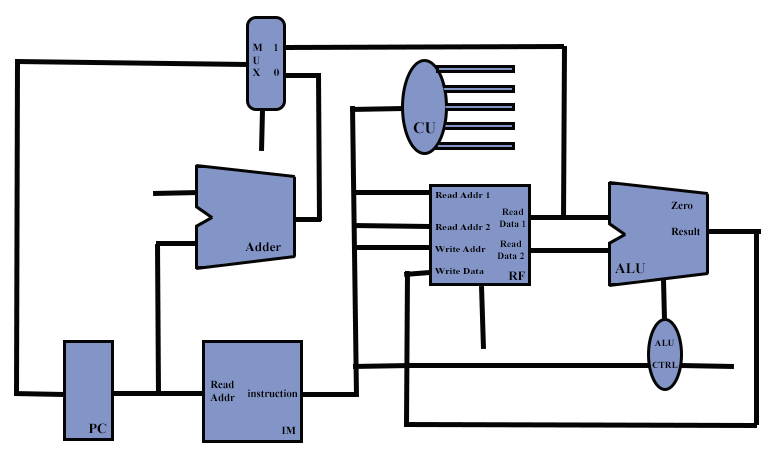
\includegraphics[scale=0.6]{add2.png}
\\
\pagebreak
\\
\textbf{addi:}\\
\\
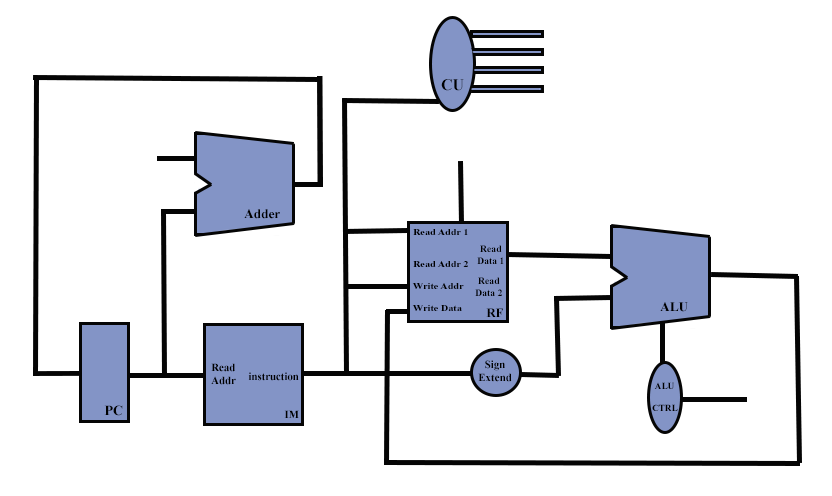
\includegraphics[scale=0.6]{addi2.png}
\\
\\
When \textit{add} operation is being executed, first the instruction is read from memory with the help of \textit{PC}, therefore the \textit{PC} adder is shown. Since the data is read from two source registers, \textit{RegDst} is activated. \textit{WriteReg} is also signaled, since we are writing to a register. \textit{ALUSrc} is deactivated at this time. \textit{ALUSrc} determines the datapath so that both values from the source registers are put into the ALU where the operation is executed and then written to the destination register.\\
\\
When \textit{addi} operation is being executed, first the instruction is read from memory with the help of \textit{PC}, therefore the \textit{PC} adder is shown. \textit{RegDst} is deactivated. The binary value flows through the sign-extend component and into the multiplexer where the \textit{ALUSrc} being activated this time, leads the bits into the ALU along with the value from one of the source registers. Then, The operation is executed in the ALU and it is written back in the register.  \\
\\
\problem{}{0}
\\
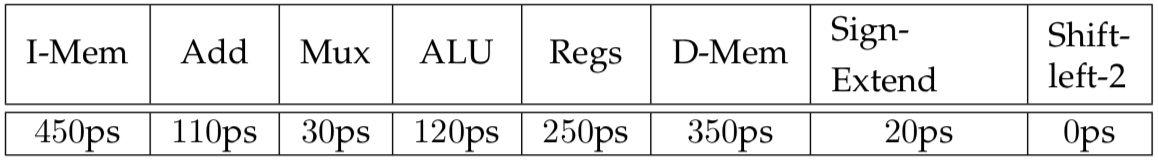
\includegraphics[scale=0.35]{2.png}\\
\\
\textbf{a) What is the clock cycle time, if the only type of instruction we need to support are the ALU instructions \textit{(add, and, etc.)}} \\
\\
\solution
For instructions like \textit{add, and, etc.} the following logic blocks are activated:\\ \textbf{I-Mem, Regs (RegF), Mux2, ALU, Mux3, Regs (RegF)}.\\ 
Thus, the clock cycle time will be: $450+250+2\times 30+120+3\times 30+250=\mathbf{1220ps}$
\\
\\
\pagebreak
\\
\textbf{b) What is the clock cycle time, if we only have to support \textit{sw} instructions?}\\
\\
\solution
The execution of \textit{sw} would follow the following steps in your diagram:\\ \\
1. Instruction is read and decoded from the PC in the Instruction Memory subcircuit.\\
2. The register file is read for \$rs and \$rt (Registers subcircuit)\\
3. The value of \$rs is added to the sign extended immediate (selected by ALUSrc) (ALU subcircuit).\\
4. The added value and \$rt are passed to the Data Memory subcircuit where the value of \$rt is written to memory.\\
\\ 
Thus, the following logic blocks are activated: \textbf{I-Mem, Regs, ALU and D-Mem}\\
The clock cycle time will be: $450+250+120+350=\mathbf{1170ps}$\\
\\
\textbf{c) What is the clock cycle time, if we have to support add, beq, lw, and sw instructions?}\\
\\
\solution
Whenever we have \textit{sw, lw, add, beq} instructions, \textit{lw} is the longest possible time-consuming instruction path, the following logic blocks are activated:\\
\textbf{I-Mem, Regs (RegF), ALU, D-Mem, Mux3, Regs (RegF).}\\
The clock cycle time will be:
$450+250+120+350+3\times 30+250=\mathbf{1510ps}$
\end{document}